\section{如何使之具体？}\label{sec:4}

在这一节，我们的叙述在一条（余）切丛的岔路上分出去——简要谈谈 Hitchin 可积系统，它使几何朗兰兹的许多部分变得远为几何、远为具体。

\subsection{阿贝尔化，或希格斯机制}\label{sec:4.1}

微局部分析的一个重要教训是：函数的行为更接近相空间的几何（Wigner 分布、波前集以及偏微分方程的特征线都住在这里），而不只是位置空间的几何。因此，要理解如何在 $\Bun_{G}$ 上（乃至为何要）做调和分析，我们确实应当问：它的余切丛 $T^{*}\Bun_{G}$ 有什么特殊之处？图~\ref{fig:3} 给出了图示。

丛的模空间的余切丛本身也有模空间的解释，即 $G$-希格斯丛的模空间
\[
\Higgs_{G}(C)=\{P\in\Bun_{G},\ \eta\in\Gamma(C,\mathrm{ad}^{*}(P)\otimes\Omega^{1}_{C})\}:
\]
这些是丛连同希格斯场（Higgs field）的数据，后者是取值于自同态的一形式（共伴随丛扭以 $C$ 上的一形式所得的截面）。我们同样把 $\Higgs_{G}$ 当作模叠处理，并注意它像 $\Loc_{G}$ 一样轻度奇异。与 $\Bun_{G}$ 一样，它也有一个配对的子商，即半稳定希格斯丛的模空间；其研究由 Hitchin~[Hit87a] 开创，是 Corlette~[Cor88] 与 Simpson~[Sim92] 的非阿贝尔 Hodge 对应的主题。

作为余切丛，$\Higgs_{G}$ 有自然的辛结构（借助非阿贝尔 Hodge 理论，它在相应的半稳定模空间上细化为超 Kähler 结构）。Hitchin~[Hit87b] 发现它还带有一种华丽而稀有的几何结构，即完全可积的 Hamilton 系统；后者的诸实例还原了许多被研究得最多的可积系统。为简单起见，我们聚焦于 $G=\mathrm{GL}_{n}$ 的情形，尽管整个理论对其他群也有漂亮的推广，见~[DM96, DG02]。具体说，取取值于自同态的一形式的特征多项式，定义了一个映射
\begin{equation}\label{eq:hitchin}
\Hitch:\Higgs_{n}\longrightarrow\bigoplus_{i=1}^{n}\Gamma(C,\Omega^{\otimes i}_{C})
\end{equation}
从希格斯丛的模空间到一个向量空间。这个映射是 Lagrangian 纤维化，而一般纤维 $\Hitch^{-1}(\chi)$ 的连通分支是复环面（阿贝尔簇），如图所示。

事实上，一般纤维实际上是曲线上的 Picard 群（线丛的模空间）。希格斯场 $\eta$（作为取值于矩阵的一形式）的本征值切出一条曲线 $C_{\eta}\subset T^{*}C$，它是 $C$ 的 $n$ 重覆叠，称为谱曲线（spectral curve）。谱曲线的数据等价于特征多项式 $\chi(\eta)$ 的数据，所以我们可以把映射 $\Hitch$ 看作 $\eta\mapsto C_{\eta}$。纤维于是描述固定本征值下可能的诸本征空间；一般情形下它们是谱曲线上的一个线丛——因此纤维被等同于 Picard 群 $\Hitch^{-1}(\chi(\eta))=\mathrm{Pic}(C_{\eta})$。

另一方面，零纤维 $\Nilp=\Hitch^{-1}(0)$——整体幂零锥~[Lau88]——由 $\eta$ 为幂零矩阵的希格斯场构成（见图）。这是一个可约簇，包含零截面 $\Bun_{G}\subset\Nilp\subset T^{*}\Bun_{G}$ 作为希格斯场恒为零的那个不可约分支。

换言之，Hitchin 纤维化把 $\Bun_{G}$ 呈现为某条曲线的 Picard 群之退化中的一个分支——所以 $\Bun_{G}$ 在骨子里非常接近阿贝尔簇，就像 $\mathrm{GL}_{1}$ 的情形一样。这一 $\Bun_{G}$ 的阿贝尔形变背后的想法，是规范场论中著名的、用于质量生成与对称性自发破缺的希格斯机制之变体的几何实现：在那里，希格斯场 $\eta$（它带规范荷）取真空期望值 $\Hitch(\eta)$，从而把规范对称性破缺为 $\eta$ 的中心化子。

更引人注目的是，GLC 的谱侧与自守侧现在开始看起来非常相似：毕竟，向量丛上的联络是取值于自同态的一形式的扭曲版本。具体说，模空间 $\Loc^{\dR}_{\Gd}$ 在一个单参数族中退化到 $\Gd$-希格斯丛的空间 $\Higgs_{\Gd}=T^{*}\Bun_{\Gd}$。Hausel–Thaddeus~[HT03] 与 Donagi–Pantev~[DP12] 的发现是：Langlands 对偶群的 Hitchin 系统一般地构成同一向量空间上互为对偶的阿贝尔簇族——用物理的语言说，它们互为 SYZ 镜像（见近期的综述~[Hau23]）。确实，[DP12] 证明：在 Hitchin 基上的一般点处，有一个等价，即 Dolbeault GLC
\begin{equation}\label{eq:dolbeault}
\QCoh(\Higgs_{G})\ \longleftrightarrow\ \QCoh(\Higgs_{\Gd}),
\end{equation}
它在纤维上由对偶阿贝尔簇上凝聚层的傅里叶–Mukai 变换~[Muk81] 的变体给出。（这个等价的适用范围随后在~[Ari13, MRV19a, MRV19b] 中被扩展，尽管关于整个 Hitchin 系统的完整图景仍未可得。）这提示 GLC 应当物理地表现为（同调）镜像对称的一种形式，而这确实在~[KW07] 中得到确认。

\begin{figure}[htbp]
\centering
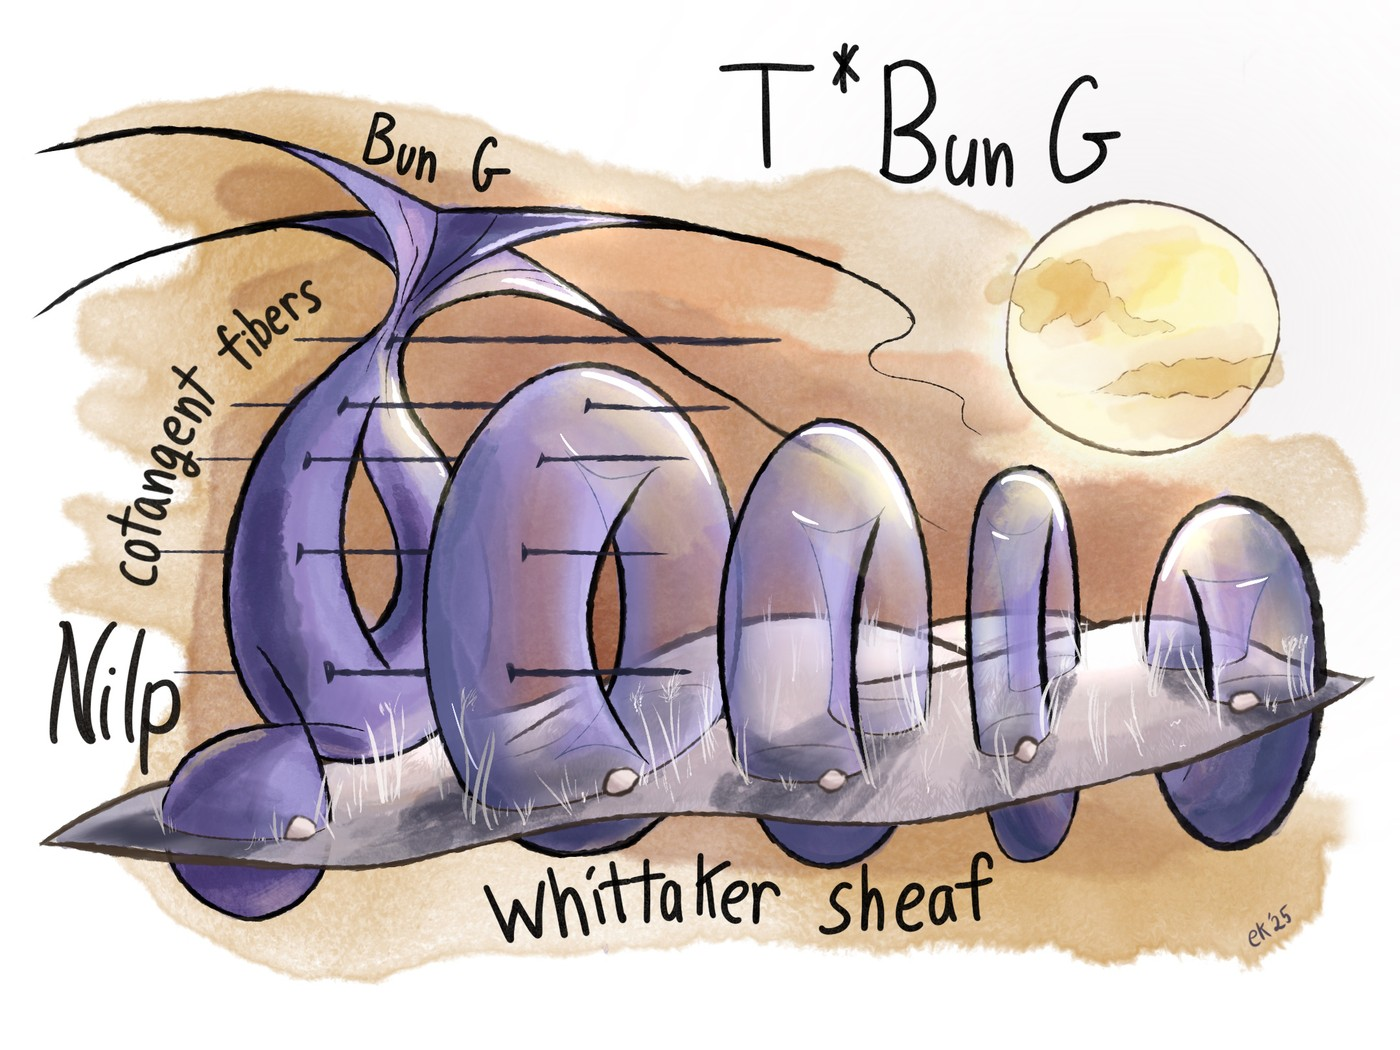
\includegraphics[width=0.78\linewidth]{figures/fig3.jpg}
\caption{希格斯丛模空间的 Hitchin 纤维化，图示零纤维（幂零锥，含 $\Bun_{G}$）与 Hitchin 截面（Whittaker 层的微支撑）。}
\label{fig:3}
\end{figure}

\subsection{层的阿贝尔化}\label{sec:4.2}

Hitchin 系统的几何与自守层理论有何关系？代数分析给出的一个重要洞见是：层就像广义函数一样，本质上具有微局部的性质，其支撑落在相空间中。因此，如 Donagi 首先建议的那样，我们可以用“阿贝尔化”的途径来处理 GLC：借助 Hitchin 纤维化的几何，把 $\Bun_{G}$ 上的层论“一般地”化归为 $\mathrm{GL}_{1}$ 的情形。\zhnote{“微局部”与“奇异支撑”是这块内容的技术核心：一个层（或 D-模）的奇异支撑是相空间 $T^{*}X$ 中的子簇，记录函数（层）在哪些点与哪些方向上不光滑、不“光滑可延拓”，它是物理中波前集的代数对应物；对 D-模而言它与特征簇在 Riemann--Hilbert 对应下相合。nLab 的 \emph{singular support} 页面实际重定向到“分布的支集”，义项不同，故此处不作链接；相关概念可自上而下的入口是 \emph{characteristic variety} 词条，\href{https://ncatlab.org/nlab/show/characteristic+variety}{\texttt{https:/\allowbreak{}/\allowbreak{}ncatlab.\allowbreak{}org/\allowbreak{}nlab/\allowbreak{}show/\allowbreak{}characteristic+\allowbreak{}variety}}（最后修订 2017-08-29）。}

图景如下：在傅里叶理论中，单色波（指数函数 $e^{i\lambda x}$）在动量空间中是局部化的，因此在微局部看来像 $\mathbb{R}^{2}_{x,t}$ 中的直线 $\{t=\lambda\}$。同样，我们可以期望所求的本征层——$\Bun_{G}$ 上的“单色”层——沿 Hitchin 纤维微局部地局部化，从而可以通过阿贝尔对偶来把握。把 Hitchin 纤维替换为它们在余切丛中按伸缩取极限后的版本，我们得到这一陈述的一个更粗糙的渐近版本：本征层应当以整体幂零锥 $\Nilp=\Hitch^{-1}(0)$ 为其特征簇~[Lau87]。（这在很大程度上解释了为什么在 Betti GLC 的表述中，带有幂零奇异支撑的层是应当考虑的正确推广（\S\ref{sec:2.5}））。

在他们引入我们所知的 GLC 的巨著~[BD] 中，Beilinson 与 Drinfeld 证明：Hitchin 的 Hamilton 量（$\Bun_{G}$ 上由 Hitchin 基上线性函数拉回的函数）可以形变为 $\Bun_{G}$ 上整体定义的交换微分算子\anote{差一个由自旋结构给出的扭。}。这些微分算子的本征系统给出 $\Bun_{G}$ 上一族整体定义的微分方程组（D-模），它们在微局部对应于 Hitchin 纤维上的常值层（不带任何缠绕）。它们是 \S\ref{sec:1.3} 中 $C^{\times}$ 上微分方程 $z\frac{d}{dz}f=sf$，以及 \S\ref{sec:2.4.1} 中雅可比簇上整体定义的 D-模族 $\{t_{\xi_{i}}f=\mu_{i}f\}_{i=1}^{g}$ 的非阿贝尔推广。

此后出现了若干把 GLC 的大部分阿贝尔化的途径：

\begin{itemize}
\item \textbf{渐近展开}：第一，微分算子有半经典极限，此时它们退化为其象征（symbol），即相空间上的函数。这提示了下述由 Arinkin~[Ari05] 发展的想法：
\begin{equation}\label{eq:asymp}
\Dmod(\Bun_{G})\ \rightsquigarrow\ \QCoh(\Higgs_{G})\ \longleftrightarrow\ \QCoh(\Higgs_{\Gd})\ \rightsquigarrow\ \QCoh(\Loc_{\Gd}).
\end{equation}
过渡到象征把 $\Bun_{G}$ 上的 D-模退化为 $\Higgs_{G}$ 上的拟凝聚层。然后我们用 Dolbeault GLC \eqref{eq:dolbeault} 从 $\Higgs_{G}$ 过渡到 $\Higgs_{\Gd}$，最后从 $\Higgs_{\Gd}$ 形变到 $\Loc_{\Gd}$。这给出了 GLC 的一个“一般的、形式渐近的”片段。
\item \textbf{谱侧的阿贝尔化}：上述联络的形式 WKB／半经典描述有一个引人注目的整体形式，由 cluster 簇的理论与超对称量子场论~[FG06, GMN13] 提供。这用环面坐标卡给出了局部系统空间 $\Loc_{\Gd}$ 的阿贝尔化描述，而这些卡来自覆叠空间上的秩一局部系统。
\item \textbf{模 $p$ 约化}：把微分算子模素数 $p$ 约化也有经典极限的效果（因为 $p$ 次导数模 $p$ 消失，于是环 $D$ 模 $p$ 变得非常接近其象征）。结果是可以把 $C$ 上的平坦联络与 $\Bun_{G}$ 上的 D-模直接与它们的 Dolbeault 对应物联系起来。这给出了 de Rham GLC 的模 $p$ 形式中一般部分的证明，其方法是约化到 Dolbeault 情形，如~[BB07, CZ17] 所完成的那样。
\item \textbf{Fukaya 范畴与微局部层}：Kapustin–Witten 提议把自守层放在辛几何与镜像对称的语境中看作 $T^{*}\Bun_{G}$ 上的 A-膜，即 Fukaya 范畴的对象。这些对象恰好由配备局部系统的 Lagrangian 表示。其中包括带局部系统的 Hitchin 纤维，它们给出了 Hecke 本征层的具体几何实现。这对后来借助微局部层论~[NZ09, Nad09, Kon09, GPS24] 理解 Fukaya 范畴产生了巨大影响。我们将看到这些想法出现在 GLC 的证明中（\S\ref{sec:5.4}）。
\item \textbf{非阿贝尔 Hodge 理论}：最后，非阿贝尔 Hodge 理论（由 Simpson、Mochizuki 等人发展）导向一种关于 GLC 的深刻视角，正由 Donagi–Pantev–Simpson 发展（综述见~[DP09]，另见~[DP22, DPS24]）。簇 $X$ 上的非阿贝尔 Hodge 对应用调和映射理论把合适的平坦联络、或更一般的 D-模，与希格斯层、即 $T^{*}X$ 上的凝聚层等同起来。$C$ 上的非阿贝尔 Hodge 理论造就了希格斯丛与局部系统模空间深刻的超 Kähler 几何，而 $\Bun_{G}$ 上的非阿贝尔 Hodge 理论则直接从 Hitchin 纤维上的线丛（视为希格斯层）构造出特殊的 Hodge（或 twistor）D-模。这为完成 \eqref{eq:asymp} 中从局部系统到 D-模的翻译提供了另一条途径。另见 \S\ref{sec:6.2}。
\end{itemize}
